
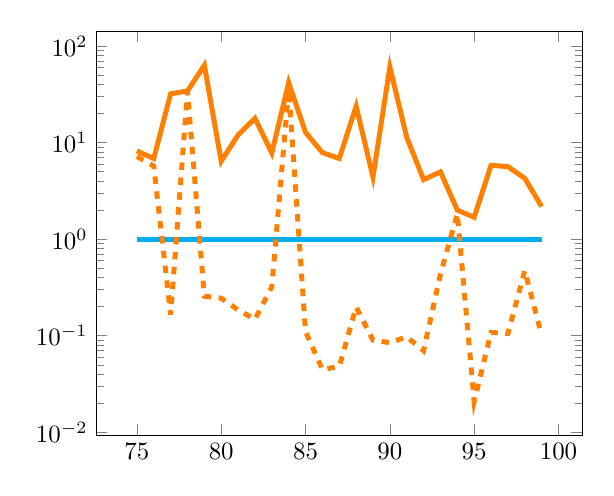
\begin{tikzpicture}[scale=0.9]
\begin{semilogyaxis}
\addplot[color=cyan,line width=2pt] coordinates {(75,1.0)(76,1.0)(77,1.0)(78,1.0)(79,1.0)(80,1.0)(81,1.0)(82,1.0)(83,1.0)(84,1.0)(85,1.0)(86,1.0)(87,1.0)(88,1.0)(89,1.0)(90,1.0)(91,1.0)(92,1.0)(93,1.0)(94,1.0)(95,1.0)(96,1.0)(97,1.0)(98,1.0)(99,1.0)};
\addplot[color=orange,line width=2pt] coordinates {(75,8.191162127116824)(76,6.85100611958098)(77,32.0508551783438)(78,34.29346093896873)(79,63.343089068426224)(80,6.417660024237365)(81,12.007284036447668)(82,17.841775943947198)(83,7.839200794413155)(84,41.71054949080286)(85,12.776348650663557)(86,7.879975235861888)(87,6.8435075194053425)(88,23.75571229789159)(89,4.408615988139119)(90,60.665412747281316)(91,11.350741058663615)(92,4.136189630494718)(93,4.977347919705271)(94,1.9997786099708064)(95,1.6845750855229675)(96,5.826392367631751)(97,5.633381221659809)(98,4.265889518572248)(99,2.1795873015873015)};
\addplot[dashed,color=orange,line width=2pt] coordinates {(75,7.174075130306077)(76,5.724735312725705)(77,0.1656162296104133)(78,34.04332499677094)(79,0.25646323732974474)(80,0.2450273164119857)(81,0.18480211600507787)(82,0.1476968958336536)(83,0.32051016306904273)(84,36.103729762248065)(85,0.110410655951058)(86,0.04462510878270693)(87,0.0480465873652593)(88,0.19814778011325135)(89,0.08989254496974654)(90,0.08465797914316582)(91,0.09719879702909902)(92,0.06998198960560043)(93,0.4326533828408048)(94,1.8403261938175894)(95,0.02082720144660793)(96,0.10826261673232754)(97,0.10515546659185705)(98,0.4708499460744553)(99,0.10117318171049514)};

\end{semilogyaxis}
\end{tikzpicture}
